% Copyright (c) 2014,2016 Casper Ti. Vector
% Public domain.

\chapter{研究方法概述}\label{chap:2}
\section{RADYN代码}
我们采用了一维辐射流体力学模拟代码RADYN\parencite{Carlsson1992,Carlsson1997,Allred2005,Allred2015}来模拟低层大气在沿耀斑环向下传播的非热电子加热时的动力学演化过程。RADYN代码是由挪威奥斯陆大学(\textit{University of Oslo})的Mats Carlsson教授于上世纪90年代开发的流体力学代码,其最主要的特点是能够考虑非局部热动平衡和非平衡电离下的辐射转移过程。最早它被运用于研究在明亮米粒组织结构是如何被低层激波加热的,成功再现了米粒组织上的Ca \textsc{ii} H和K线的Doppler频移震荡现象\parencites{Carlsson1997}。90年代末美国华盛顿大学(\textit{University of Washington})的Suzanne L. Hawley教授意识到了其在模拟耀斑等剧烈的大气动力学过程中的潜力,并和其他研究者合作将其开发为能够模拟非热电子加热低层大气的辐射流体力学代码。\textcites{Abbett1999}率先在RADYN代码中加入了非热电子加热,软X射线加热以及来自于轫制辐射和金属碰撞激发造成的光学薄辐射冷却等过程,对耀斑的爆发相进行了模拟。\textcites{Allred2005}拓展了代码的应用范围,使其同样可以用于模拟M矮星上同样由非热电子作为低层大气加热机制的耀斑。随后RADYN代码又新增了Fokker-Planck方程来计算非热电子加热,非热电子撞击硬靶(\textit{thick target})产生返回电流对日冕的加热\parencites{Allred2015},更加精确的Balmer线系线性Stark效应的致宽\parencites{Kowalski2017b}等一系列新的特征,对耀斑爆发过程进行了更加细致的模拟。下面我们对主要的物理过程及其数值处理方法做一个简介,涉及代码内部计算的公式全部引自\textcites{Allred2015}。

\subsection{流体力学及辐射转移方程组}
RADYN代码采用求解一维流体力学及辐射转移方程组的方法来模拟太阳耀斑爆发时低层大气的动力学演化。其主要方程组如下\parencites{Allred2015}:

\begin{gather}
	\frac{\partial \rho}{\partial t}+\frac{\partial \rho v}{\partial z}=0 \\
	\frac{\partial \rho v}{\partial t}+\frac{\partial \rho v^{2}}{\partial z}+\frac{\partial\left(p+q_{\mathrm{v}}\right)}{\partial z}+\rho g-A_{\mathrm{beam}}=0  \\
	\frac{\partial \rho e}{\partial t} +\frac{\partial \rho v e}{\partial z}+\left(p+q_{\mathrm{v}}\right) \frac{\partial v}{\partial z} +\frac{\partial\left(F_{\mathrm{c}}+F_{\mathrm{r}}\right)}{\partial z}-Q_{\mathrm{cor}}-Q_{\mathrm{beam}}-Q_{\mathrm{rc}}=0 \\
	\frac{\partial n_{i}}{\partial t}+\frac{\partial n_{i} v}{\partial z}-\left(\sum_{j \neq i}^{N^{\prime}} n_{j} P_{j i}-n_{i} \sum_{j \neq i}^{N^{\prime}} P_{i j}\right)=0 \\
	\mu \frac{\partial \boldsymbol{I}_{\nu \mu}}{\partial z}=\eta_{\nu \mu}-\chi_{\nu \mu} \boldsymbol{I}_{\nu \mu}
\end{gather}
其中,$z$, $e$, $\rho$, $v$和$p$分别代表高度、内能密度,密度,一维速度和压强。$g$是重力加速度,$q_v$是粘性项。$F_c$为对流热流,$F_r$为辐射通量。$P_{ij}$是能级$i$到$j$之间的跃迁频率,包含了碰撞跃迁频率$C_{ij}$与辐射跃迁频率$R_{ij}$。辐射转移方程为一维平面平行层形式,能量方程中的辐射通量$F_r$由$\boldsymbol{I}_{\nu\mu}$在立体角上积分得到。$Q_{cor}$是一个人工的日冕加热项。$Q_{\mathrm{beam}}$和$A_{\mathrm{beam}}$是由于入射入射非热电子带来的能量和动量。

\subsection{光学厚与光学薄辐射转移}
对于光学厚的辐射转移,RADYN会详细计算部分原子部分能级的NLTE下的能级平衡和辐射转移方程。这些原子包括一个6能级的氢原子模型,一个9能级的氦原子模型,一个6能级的Ca \textsc{ii}离子模型和一个4能级的Mg \textsc{ii}原子模型。剩下原子造成的不透明度将会采用\textcites{Gustafsson1973}的代码在LTE的假设下处理,给出一个依赖于温度、密度和频率的不透明度函数。对于日冕中不同温度成分的光学薄辐射造成的能量损失,由CHIANTI原子数据库\parencites{Dere1997,Landi2013}计算得出。
\subsection{加热机制}
这里主要介绍模型中三种主要的加热机制和它们的处理方法:

\textbf{非热电子束加热}\ \ RADYN代码考虑了相对论效应,Coulomb碰撞,回旋同步辐射,投掷角散射和磁场梯度效应,采用一个Fokker-Planck方程来描述非热电子的能量分布函数$f(E,\mu,z)$\parencites{Allred2015}
\begin{multline}
	\mu \frac{\partial \Phi}{\partial z}-\frac{d \ln B}{2 d z} \frac{\partial}{\partial \mu}\left[\left(1-\mu^{2}\right) \Phi\right] =\frac{1}{\beta^{2}} \frac{\partial}{\partial E}\left\{\left[C+S \beta^{3} \gamma^{2}\left(1-\mu^{2}\right)\right] \Phi\right\} \\
	-\frac{S}{\beta \gamma} \frac{\partial}{\partial \mu}\left[\mu\left(1-\mu^{2}\right) \Phi\right] +\frac{C^{\prime}}{\beta^{4} \gamma^{2}} \frac{\partial}{\partial \mu}\left[\left(1-\mu^{2}\right) \frac{\partial \Phi}{\partial \mu}\right]+\frac{\Sigma}{c \beta^{2}}
\end{multline}
其中,$\beta$为离子的相对论因子,$\Phi = f/\beta $,$\gamma = E+1$是无量纲化的相对论性总能量。$\Sigma$是电子从环顶入射的源项,$C$与$C'$是描述电子能量损失和投掷角扩散的因子,$S$是用来描述电子同步回旋辐射能量散失的因子。这些参数的具体形式参见\textcites{Allred2015}。RADYN代码将计算在电子和带电粒子、中性粒子相互作用散失能量时的分布函数变化,同时给出非热电子对局部大气的加热。

\textbf{XEUV逆加热(EUV backwarming)}\ \ 由于耀斑过程中会产生低层大气中的X射线和EUV辐射,这些高能光子同样也会重新通过光致电离等过程重新加热低层大气。这些加热在RADYN代码中都依靠CHIANTI原子数据库给出的发射系数确定。

\textbf{返回电流加热(return current heating)}\ \ 显然当一系列非热电子沿耀斑环向下传播时会形成一个向上的宏观电流,这个电流同样会贡献出焦耳加热项。在同时考虑入射电子热和非热成分后,RADYN代码采用如下公式来计算返回电流加热\parencites{Allred2015}:
\begin{equation}
	Q_{\mathrm{rc}}(x)=\begin{cases}\eta e^{2} F_{\mathrm{e}}^{2} & x<x_{rc} \\ {\eta e^{2} F_{\mathrm{e}}^{2}\left(\delta \frac{E_{\text { therm }}}{E_{\mathrm{c}}}+\frac{V(x)}{E_{\mathrm{c}}}\right)} \\ { \times\left(\frac{E_{\text { therm }}}{E_{\mathrm{c}}}+\frac{V(x)}{E_{\mathrm{c}}}\right)^{1-2 \delta}} &x\geq x_{rc} \end{cases} 
\end{equation}
其中$\eta$是电阻率,$F_e$是电子束通量,$\delta$是非热电子分布谱指数,$E_c$是非热电子截止能量。$x$为据环顶的距离,$x_{rc}$是电子被完全热化时距环顶的距离。一般来说,返回电流会让非热电子束在日冕中耗散更多的能量。
\subsection{初始输入}\label{sec:2.1.4}
在运行RADYN代码时,主要调节的参数是入射非热电子束的参数和初始大气条件。下面主要介绍的是比较重要的参数:

\textbf{电子束参数}\ \ RADYN输入中要求提供程序运行各时间点从环顶入射的非热电子束的参数,一般包括非热部分的谱指数$\delta$,截止能量$E_c$与总能量通量。一般来说,更大的截止能量$E_c$会让电子束在更深的大气中耗散大部分能量。而更大的谱指数(谱更加硬了)$\delta$会让电子束在低层大气中有更大的加热率。一般来说截止能量$E_c$设置在几十KeV,而谱指数$\delta$一般在3-6左右,能量通量根据模拟耀斑的等级不同而不同,对于太阳耀斑一般在$10^8-10^{12}\ \mathrm{erg\  cm^{-2}\  s^{-1}}$左右。

\textbf{初始大气}\ \ 
为了模拟一维耀斑环在电子束入射之前的初始大气状态,RADYN提供了一系列的初始大气。一般来说初始大气包含几个特征参数:光球层温度、耀斑环长度、日冕电子密度和日冕温度。光球层温度一般在$5000-5800$ K,耀斑环长度在$10-100$ Mm之间,日冕电子密度一般在$10^8\ \mathrm{cm^{-3}}$量级,日冕温度在MK量级。此外,RADYN还提供了一个M矮星的初始大气用于恒星耀斑的模拟,其拥有较低的光球层温度($\sim 3500$ K)和较高的日冕电子密度($10^{10}\ \mathrm{cm^{-3}}$)和温度。
\section{RH代码}
RH代码\parencites{Uitenbroek2001}是一套利用基于多能级加速$\Lambda$迭代(\textit{multi-level accelerated lambda iteration, MALI})方法计算给定大气中NLTE辐射转移过程的代码。整套方法基于\textcites{Rybicki1991},但考虑了PRD效应的影响。在这篇文章中,我将使用RH代码的MPI版本,RH1.5D代码\parencites{Pereira2015b}来求解耀斑大气中的辐射转移过程。RH1.5D代码支持并行计算多个一维大气模型中的辐射转移过程,能够大大加快计算速度。同时,RH1.5D代码还支持使用\textcites{Leenaarts2012}中描述的散射过程中各向异性PRD的近似算法,对模拟Mg \textsc{ii}等一系列由散射形成的谱线能得到比较好的结果。RH代码的一个缺点是假设辐射转移过程中原子能级占据数是统计平衡假设下的,即能级粒子数不随时间变化,这在耀斑这样剧烈爆发的模拟中可能并不是很好的假设\parencites{Abbett1999,Rubio2017}。

\subsection{求解过程}
限于篇幅和作者能力有限,我们在此不再详细叙述RH内部计算辐射转移过程的具体公式,仅对整个迭代求解过程做一个简单介绍。首先,代码将建立所有计算波长点和跃迁能级的列表;之后将建立一个能级上粒子数分布的初始解,可以是基于LTE情况下的,也可以是基于无辐射场情况下的;之后基于给定的原子能级数和一个给定的发射吸收谱线强度比$\rho$,计算出在PRD情况下的辐射场参数;之后在基于固定的原子能级数的情况下,重新计算发射吸收谱线强度比$\rho$。最后这两步可以持续迭代,直到前后两步得到的平均辐射强度的相对差异小于设定的阈值。

\subsection{输入输出}
接下来我们简单介绍一下RH1.5D代码支持的输入和输出参数。为了让代码能够正常运行,需要输入的大气参数是:(一维)温度分布,电子密度分布,氢原子能级粒子数分布,宏观速度分布,微观湍动速度分布和各个格点的高度。如果需要计算Stokes参数,还需要给出磁感应强度矢量的分布。同时可以在\texttt{atoms.input} 文件中输入文件中指定在模拟中使用的原子,跃迁能级和是否当作LTE背景不透明度处理。在\texttt{ray.input}文件中可以指定求解辐射转移方程的方位角$\mu$和需要详细输出辐射转移波长的波长点。在\texttt{keyword.input}文件中还有一系列代码选项,如收敛阈值、是否使用大气波长、是否输出$\tau=1$的高度,是否需要去除某个温度以上的所有大气方便计算和是否计算Stokes参量等可供修改。在输出文件中,主要包含了辐射强度$I_{\nu}$,各原子能级粒子数等,如果使用了Stokes模式,还会有$UVQ$等一系列参量,如果在\texttt{ray.input}中指定了波长点,还可以输出这些波长点的不透明度$\chi_\nu$和源函数$S_\nu$等与辐射场有关的参量。
\subsection{Stark致宽效应处理}\label{sec:2.2.3}
为了呼应后面介绍的Stark-B数据库,我们在这里简单介绍一下RH代码中对于非氢原子的二次Stark效应致宽的计算方法。计算Stark致宽效应的经典方法主要有两种,一种是碰撞理论(\textit{impact theory},\cites{Weisskopf1932}),另一种是统计理论(\textit{statistical theory},\cites{Holtsmark1919})。前者的物理图像是每次与带电粒子的碰撞会打断辐射粒子的辐射,经过Fourier变换后非无穷长的波列将会在频域空间有一定的展宽,最后将会得到一个Lorentzian形的谱线。而后者则同时考虑多个带电粒子在辐射粒子周围的统计分布,在带电粒子和辐射粒子相对静止的假设下,计算他们的电场对辐射粒子能级的扰动,最后会得到一个Holtsmark分布。一般来说,对于自由电子的Stark致宽而言,碰撞理论能够得到比较好的结果,对于一条较宽的谱线而言,在线心周围碰撞效应的近似比较好,而在线翼部分统计理论的效果比较好,关于这两种经典方法的优劣,可以参见附录\ref{sec:a.2}中对于Mg \textsc{ii}线的讨论。

RH代码采用Lindholm近似\parencites{Lindholm1945,Foley1946,Mihalas2014}下的经典碰撞理论来计算非氢原子的二次Stark效应致宽,其给出Lorentzian形谱线的半高全宽$\Gamma_{Stark}$为
\begin{equation}
    \Gamma_{Stark}=11.37C_4^{2/3}v_{rel}N_e
\end{equation}
其中$v_{rel}$为辐射粒子和带电粒子的相对速度,$N_e$为电子密度,$C_4$为Stark常数,用于衡量当一个带电粒子在距离为$r$处与辐射粒子产生作用时辐射粒子的辐射角频率改变量大小$\Delta \omega = C_4/r^4$。在RH代码中,其通过\textcites{Traving1960}中的如下公式进行计算
\begin{equation}
    C_4 = \frac{e^2 r_{bohr}^3}{4 \pi \epsilon_0 \hbar}\  \frac {\left(n_{\mathrm{effu}} \  \left(5.0  n_{\mathrm{effu}}^2 + 1.0\right)\right)^2 - \left(n_{\mathrm{effl}} \  \left(5.0  n_{\mathrm{effl}}^2 + 1.0\right)\right)^2}{18.0 \  Z^4}    
\end{equation}
其中
\begin{align}
	n_{\mathrm{effl}} &=Z \sqrt{R_{\mu} /\left(E_{c}-E_{i}\right)} \\
	n_{\mathrm{effu}} &=Z \sqrt{R_{\mu} /\left(E_{c}-E_{j}\right)}
\end{align}
$E_c$为该电离态原子的电离能,$E_i$为跃迁的低能级能量,$E_j$时该跃迁的高能级能量,$Z$为等效电荷,$R_\mu$为Rydberg常数。
\section{STARK-B数据库}\label{sec:2.3}
STARK-B数据库\parencites{STARK-B}提供了大量天体物理中重要原子谱线在周围电子和离子扰动下的致宽宽度的数据。整个数据库旨在为恒星大气和包层(\textit{envelope})提供精确计算Stark致宽效应的数据。其中主要运用半经典碰撞理论\parencites{Brechot1969a,Brechot1969b,Fleurier1977,}来计算Stark致宽效应。其中包含了带电粒子的相互作用的双曲线轨道,粒子的偶极、四极相互作用,非弹性碰撞等。对于已经计算了的跃迁,其给出$\Gamma_{Stark}$在不同温度下的值,并提供了一个拟合函数供数值模拟使用\parencites{Brechot2011}:
\begin{equation}
    \log\left(\Gamma (\mbox{{\AA}})\right) = a_0 + a_1\mathrm{Log}(T) + a_2\mathrm{Log}^2(T) 
\end{equation}

\begin{table}
	\begin{tabular}{cccccc}
	\hline
    谱线 & 跃迁 & 波长($\mbox{{\AA}}$) & $a_0$ & $a_1$ & $a_2$ \\ 
 	\hline
    Mg \textsc{ii} h& $3p\ ^2\mathrm{P}_{1/2}-3s\ ^2\mathrm{S}_{1/2}$  & 2803.53 & \multirow{2}{*}{1.13807} &\multirow{2}{*}{-1.54913} & \multirow{2}{*}{0.13423}\\ 
    Mg \textsc{ii} k& $3p\ ^2\mathrm{P}_{3/2}-3s\ ^2\mathrm{S}_{1/2}$  & 2796.35\\ 
    \hline
    Mg \textsc{ii} 2791  & $3d\ ^2\mathrm{D}_{3/2}-3p\ ^2\mathrm{P}_{1/2}$ &2791.60& \multirow{3}{*}{1.36331}& \multirow{3}{*}{-1.62649} & \multirow{3}{*}{0.15218}\\ 
    \multirow{2}{*}{Mg \textsc{ii} 2798}  & $3d\ ^2\mathrm{D}_{3/2}-3p\ ^2\mathrm{P}_{3/2}$ &2798.75\\
     & $3d\ ^2\mathrm{D}_{5/2}-3p\ ^2\mathrm{P}_{3/2}$ & 2798.82 \\
     \hline
    Si \textsc{iv} 1394& $2p^63s\ ^2\mathrm{S}_{1/2}-2p^63p\ ^2\mathrm{P}_{3/2}$  & 1393.755 & \multirow{2}{*}{-3.89461} &\multirow{2}{*}{0.65393} & \multirow{2}{*}{-0.13588}\\ 
    Si \textsc{iv} 1402& $2p^63s\ ^2\mathrm{S}_{1/2}-2p^63p\ ^2\mathrm{P}_{1/2}$  & 1402.770\\ 
    \hline
\end{tabular}
    \caption{本文中使用的STARK-B数据库数据}\label{Table1}
\end{table}

\begin{figure}
	\centering
	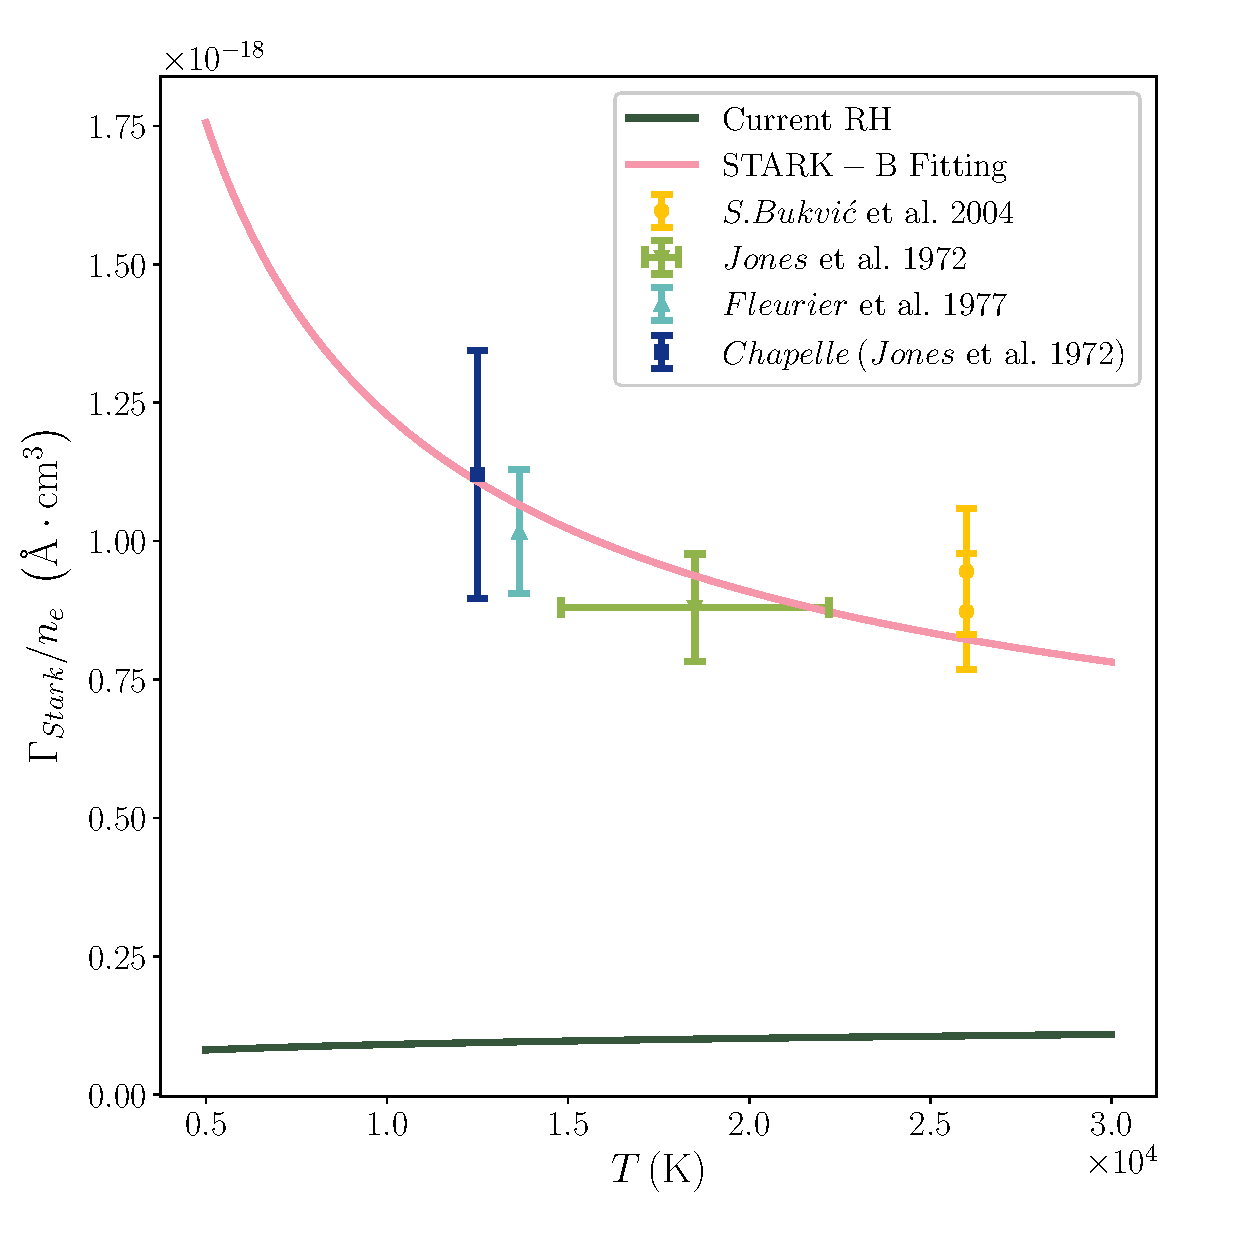
\includegraphics[width=0.6\textwidth]{figs/SB_Mg}
	\caption{RH代码与STARK-B数据库中对Mg \textsc{ii} h,k线的单位电子密度下Stark致宽宽度比较。同时我们还展示了一些实验得到的谱线致宽数据\parencites{Jones1972,Fleurier1977,Bukvic2004}。}\label{fig:2.1}
\end{figure}

\begin{figure}
	\centering
	\includegraphics[width=0.6\textwidth]{figs/SB_Si}
	\caption{RH代码与STARK-B数据库中对Si \textsc{iv}双重线的单位电子密度下Stark致宽宽度比较。}\label{fig:2.2}
\end{figure}
表~\ref{Table1}给出了本文中使用的Mg \textsc{ii}和Si \textsc{iv}线的STARK-B数据库数据。我们比较了RH代码和STARK-B数据库对Mg \textsc{ii} h,k和三重线,以及Si \textsc{iv}双重线Stark致宽效应处理结果的不同。图~\ref{fig:2.1}展示了Mg \textsc{ii} h和k线的在单位电子密度下Stark宽度随温度的变化情况。总体上来看,STARK-B数据库给出的谱线宽度和实验结果拟合的比较好,同时比RH代码给出的结果大约高了一个量级。STARK-B数据库中的宽度随温度的增加而逐步降低(由非弹性碰撞向弹性碰撞变化),但RH代码中的结果随着温度的上升而缓慢增加(粒子相对速度提高的结果)。图~\ref{fig:2.2}展示了Si \textsc{iv}双重线的结果,可以看到RH代码同样大大低估了Si \textsc{iv}双重线的Stark致宽宽度,且其对温度的依赖关系也与STARK-B数据库的数据相反。但是由于Si \textsc{iv}线的Stark宽度本来就比Mg \textsc{ii}线低大约一个量级,且在Si \textsc{iv}形成高度上电子密度也相对较低,因此其Stark致宽相对于Mg \textsc{ii}线来说应该较不明显。
% vim:ts=4:sw=4